%Alle zu bearbeitenden Felder sind als solche gekennzeichnet. 
%Warnungen sind in der Regel nicht komplett vermeidbar und auch in dieser Vorlage vorhanden (Bei mir 7). Sie sind meistens eher als Hinweise zu verstehen.
%Bei Fragen zu dieser Vorlage einfach eine Mail an gold@lfe.mw.tum.de
%Viel Erfolg!


\documentclass[
	12pt,
	headinclude,
	footinclude,
	a4paper,
	listof=totoc,
	bibliography=totoc,
	index=totoc,
	%twoside, %F�r beidseitigen Druck
	]{scrreprt}


	
	
\newcommand{\myname}[0]{Max Mustermann} %---------- HIER NAME EINTRAGEN ----------
\newcommand{\mythema}[0]{Titel der Studienarbeit} %---------- HIER TITEL EINTRAGEN ----------
\newcommand{\mythemaeng}[0]{Titel der Studienarbeit in Englisch} %---------- HIER TITEL IN ENGLISCH EINTRAGEN ----------
\newcommand{\myarbeit}[0]{Theoretische Diplomarbeit} %---------- HIER ART DER ARBEIT EINTRAGEN ----------
\newcommand{\mymodul}[0]{Produktionstechnik} %---------- HIER STUDIENGANGMODUL EINTRAGEN ----------

%----- Bitte au�erdem die Datei _names.tex anpassen ------


\usepackage[
%headinclude, 
%footinclude,
%headsepline,
%footsepline,
%plainfootsepline, 
%plainheadsepline,
automark
]{scrpage2}



\pagestyle{scrheadings}
\clearscrplain
\clearscrheadings
\ofoot[\pagemark]{\pagemark} %Seitenzahlen rechts unten, bitte!
\addtolength{\footskip}{-1cm} %Seitenzahlen ein bisschen h�her setzen


\newcommand{\bild}[4]{
  \begin{figure}[!hbt]
    \begin{center}
    %\centering
      %\vspace{1ex}
      \includegraphics[#2]{img/#1}
      \caption[#4]{\label{img.#1} #3}
    \end{center}
    %\vspace{1ex}
  \end{figure}
 }
 
%bild mit rahmen 
\newcommand{\rbild}[4]{
  \begin{figure}[!hbt]
    \begin{center}
    \fbox{
    %\centering
      %\vspace{1ex}
      \includegraphics[#2]{img/#1}
      }
      \caption[#4]{\label{img.#1} #3}
    \end{center}
    %\vspace{1ex}
  \end{figure}
 }
 
 

\newcommand{\fbild}[5]{
  \begin{floatingfigure}[r]{#5}
    \begin{center}
    %\centering
      %\vspace{1ex}
      \includegraphics[#2]{img/#1}
      \caption[#4]{\label{img.#1} #3}
    \end{center}
    %\vspace{1ex}
  \end{floatingfigure}
 }


\newcommand{\mytab}[4]{
    \begin{table}[!hbt]
    \begin{center}
      \vspace{1ex}
		\begin{tabular}{#2}
			\hline %hline here beacuse hline as first command in included \input-files produces errors
			    \input{tab/#1}
			\hline	    		
		\end{tabular}
          \caption[#4]{\label{tab.#1} #3}
    \end{center}
    \vspace{1ex}
\end{table}
}

\newcommand{\tausend}{\hspace {.5ex}} %50\t 000 => 50 000 tausender trenner 

\newcommand{\comment}[1]{} 

\newcommand{\mytabsmall}[4]{
    \begin{table}[!hbt]
    \begin{center}
      \vspace{1ex}
      {\tiny
		\begin{tabular}{#2}
			\hline %hline here beacuse hline as first command in included \input-files produces errors
			    \input{tab/#1}		
			\hline
		\end{tabular}
		}
          \caption[#4]{\label{tab.#1} #3}
    \end{center}
    \vspace{1ex}
\end{table}
}


% foldersymbol
\newcommand{\folder}[1]{
      \hspace{-3ex}
 \scalebox{0.40}[0.40]
{\includegraphics[viewport=14 15 48 48,clip]{img/folder.pdf}  }
 \bf #1 \normalfont \tiny
 }

% dokumentsymbol 
\newcommand{\dokument}[1]{
      \hspace{-3ex}
 \scalebox{0.60}[0.50]
{\includegraphics[viewport= 22 16 40 42, clip]{img/dokument.pdf}  }
 \bf #1 \normalfont \tiny
 }

% ANWENDUNGSBEISPIELE--------------------------------------------------------------------
%    \bild{meinbild.pdf}{viewport=0 0 200 350, clip=true}{BILDUNTERSCHRIFT}{Eintrag fuers Abbildungsverzeichniss}
%    \bildscale{meinbild.pdf}{viewport=0 0 200 350, clip=true}{BILDUNTERSCHRIFT}{Eintrag fuers 
% 																																									Abbildungsverzeichniss}{scalex}{scaley}
%    \mytab{datei_in_der_die_tabelle_ist.tex}{lrrr <= Format }{TABELLENUNTERSCHRIFT}{Eintrag fuers Tabellenverzeichnis}
%    \dokument[datei$.$mat] % punkt maskieren '$.$' wegen 'dirtree'-umgebung
%    \folder[mydirectory]



% macht den rand schoener (optischer randausgleich)
\usepackage[activate=normal]{pdfcprot}


\usepackage{units}
%\unit[Wert]{Einheit}
%\unitfrac[Wert]{Z�hler}{Nenner}

\newcommand{\myunit}[1]{\,\unit{#1}}  % ohne []
\newcommand{\myunitrm}[1]{\,\mathrm{\unit{#1}}} % mit []
\newcommand{\myunitfrac}[2]{\,\mathrm{\unitfrac{#1}{#2}}}
%
%U = 2.459\, 123 \myunit{V}
%\sigma = \frac{F}{A} = 133.432\, 192\, 233 \myunitfrac{N}{mm^{2}}

\usepackage{url}

\usepackage[plainpages=false,ngerman,pdfpagelabels=true,bookmarks=true, 
						%bookmarksopen=true, % waehrend testen offen lassen spaeter zumachen
						pdfpagemode={UseOutlines},pdfstartview={FitV},pdfborder={0 0 0},
						pdfauthor={\myname}, 
						pdftitle={\mythema},
						%pdfsubject={\mythema}, % optional
						%pdfkeywords={Schluesselwort1,Schluesselwort2,Schluesselwort3},
						colorlinks=true,
						linkcolor=black,
						filecolor=black,
						urlcolor=black,
						citecolor=black,
						hypertexnames=true,
						pdfpagelabels=true,
						hyperindex=true,
						linktocpage=true,
						pagebackref=true
						]{hyperref}
						
						

	\usepackage[round]{natbib}
 
	\usepackage{geometry}
%	\geometry{left=3.5cm,textwidth=15cm,top=2.5cm,textheight=24.5cm}
%	\geometry{left=2.5cm, right=2.5cm, bottom=3cm, top=2.5cm}
	\geometry{left=3cm, right=2.6cm, bottom=3cm, top=2.5cm}
	
	\usepackage{makeidx}
	\makeindex

\usepackage{setspace}
%\onehalfspacing %Zu klein im Vergleich zu Word
\setstretch{1.54} %Simuliert den 1,5 fachen Zeilenabstand von Word (Bei dieser Schriftart und dieser Schriftgr��e)
\renewcommand{\arraystretch}{1.54} %Zeilenabstand in Tabellen! 

\setlength{\parindent}{0pt} %Kein Einr�cken der ersten Zeile eines Absatzes
\setlength{\headheight}{1.1\baselineskip}

\usepackage{titlesec} %Dieser Abschnitt definiert die �berschriften
\titleformat{\chapter}[block]{\large\bfseries}{\thechapter}{.5em}{}
\titleformat{\section}[block]{\large\bfseries}{\thesection}{.5em}{}
\titleformat{\subsection}[block]{\large\bfseries}{\thesubsection}{.5em}{}
\titleformat{\subsubsection}[block]{\large\bfseries}{\thesubsubsection}{.5em}{}

%
%
%\setlength{\headsep}{1cm}
%\setkomafont{pagefoot}{\normalfont} %Sonst wird Fu�zeile kursiv
%\setkomafont{pageheadfoot}{\normalfont} %Sonst wird Kopfzeile kursiv
%
%%\pagestyle{scrheadings}
\clearscrheadfoot % clear header and footer
%\automark[section]{chapter}
%\ihead[]{\leftmark} % header left part
%%\ohead[]{\rightmark} % header right part
%\ohead[]{\scalebox{0.05}{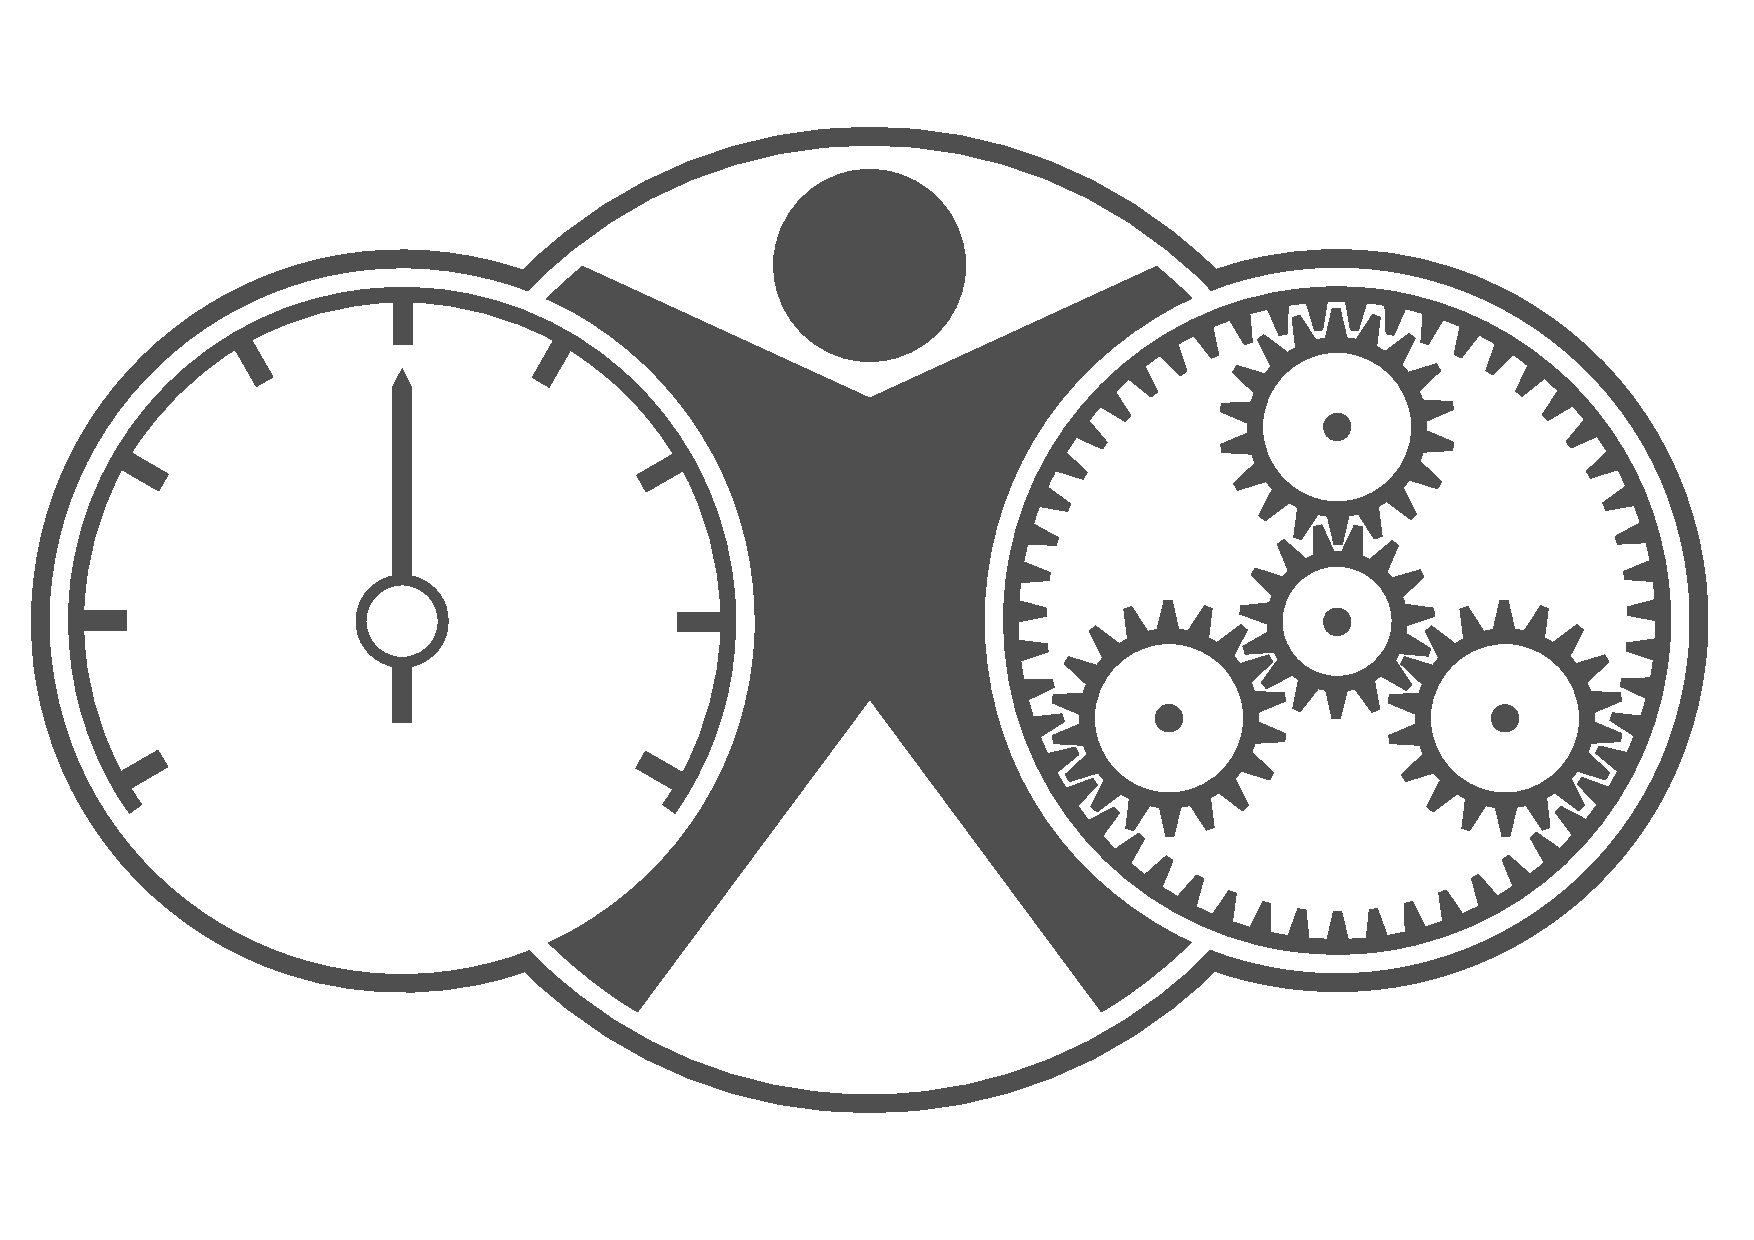
\includegraphics{img/lfe.pdf}}} % header right part
%\ifoot{\small \myarbeit \space \myname} % footer left part  
%%\cfoot{\vspace{-0.5cm}\mythema} % footer middle part
%%\ofoot{Seite\ {\pnumfont \pagemark}\ von {\pnumfont \pageref{LastPage}}} % footer right part
\ofoot{\small {\pnumfont \pagemark}} % footer right part
%\setheadsepline{0.3pt} % set header seperate line
%\setfootsepline{0.3pt} % set footer seperate line
%%\setheadwidth{textwithmarginpar}
%%\setfootwidth{textwithmarginpar}



\usepackage[dvips]{graphicx}
\usepackage{floatflt,epsfig} 

\usepackage{ngerman} % neue deutsche Rechtschreibung
\usepackage[latin1]{inputenc} % latin1-Kodierung f�r Umlaute
\usepackage[ngerman]{babel}  % Silbentrennung
\usepackage[T1]{fontenc}
\usepackage[scaled]{uarial} % Schriftart Arial
\usepackage[font=small,labelfont=it]{caption} %�berschriften kursiv


\renewcommand*\familydefault{\sfdefault} %Sonst werden die Header nicht in der entsprechenden Schriftart dargestellt
\renewcommand\thefigure{\arabic{chapter}-\arabic{figure}} %Nummerierung der Abbildungen mit - statt .
\renewcommand\thetable{\arabic{chapter}-\arabic{table}} %Nummerierung der Tabellen mit - statt .

\setcounter{secnumdepth}{3} %Tiefe der Numerierung
\setcounter{tocdepth}{3} %Tiefe des Inhaltsverzeichnisses
\usepackage{graphicx}

\clubpenalty = 10000 % Schusterjungen vermeiden
\widowpenalty = 10000 % Hurenkinder vermeiden
\displaywidowpenalty = 10000 % und nochmal f�r Formeln

\usepackage{graphicx} % Bilder
\usepackage{color} % Farben
\usepackage{colortbl} % tabellen einf�rben
\usepackage{floatflt} % graphiken mit textumfluss
\usepackage{subfigure} % graphiken nebeneinander mit (a) (b)
\usepackage[absolute]{textpos} % absolute positioning


\usepackage{scrhack}
\usepackage{listings} % programmcode als listings darstellen

%workaround
\addto\captionsngerman{
 \renewcommand{\figurename}{Abbildung}%
}

 %Definition zu Bildern und Dokumentstyle



% --------------------------------------------------
% -------------------- DOCUMENT --------------------
% --------------------------------------------------


\begin{document}


\thispagestyle{empty} %Keine Seitennummer auf der Titelseite

\begin{picture}(0,0) 
   \put(-8,0){
   
			\begin{minipage}[ht]{0.3\textwidth}
			\centering
			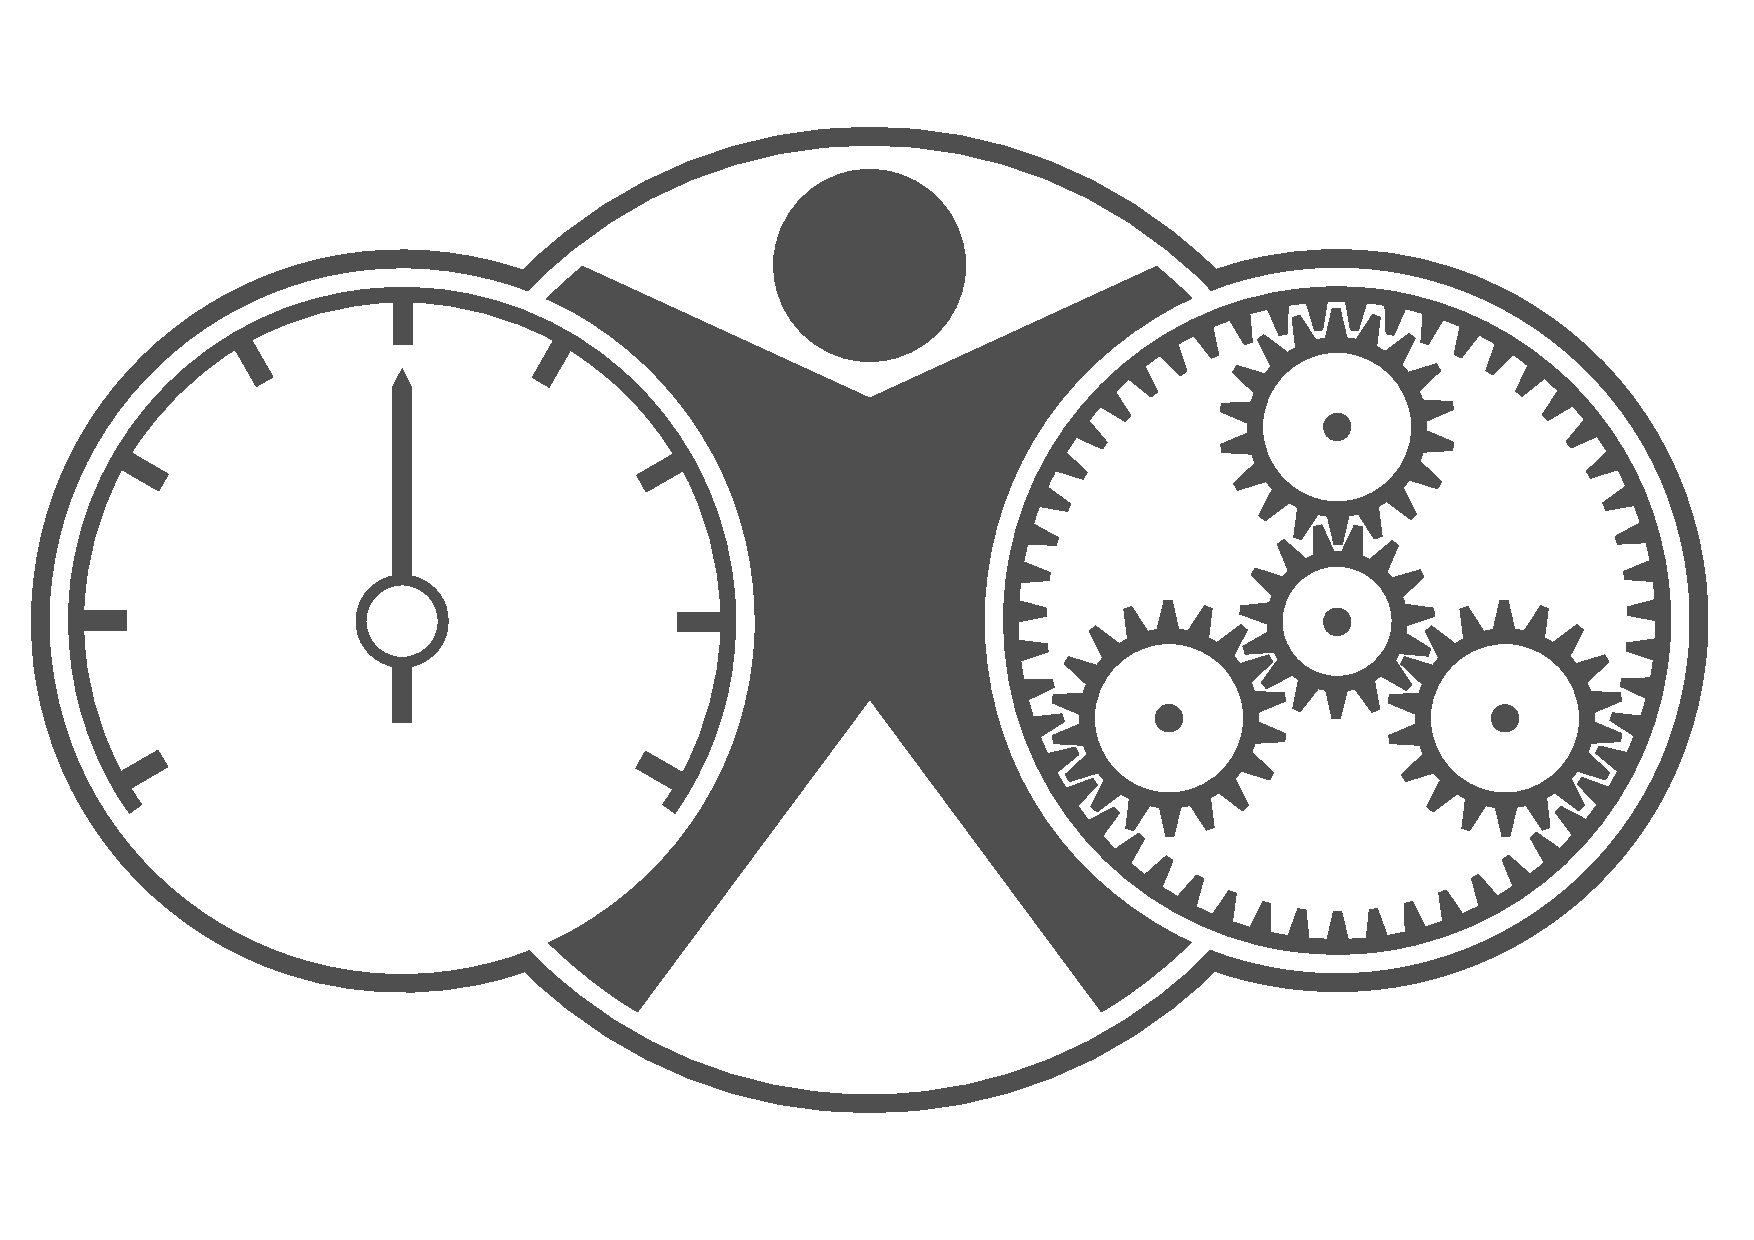
\includegraphics[width=2.5cm]{img/lfe.pdf}
			\end{minipage}
   
%   } 

   \hspace{7cm}
   
   %\put(0,0){
			\begin{minipage}[ht]{0.3\textwidth}
			\centering
			
\includegraphics[width=2.3cm]{img/tum.png}
			\end{minipage}
	}   
\end{picture} \\


\ \\
Technische Universit�t M�nchen\\
Lehrstuhl f�r Ergonomie 


\vspace{5cm}

{\large\bf \myarbeit}\\

\vspace{1cm}

{\Large\bf \mythema}\\

{\large\bf \mythemaeng}


\vspace{3cm}


{\large\bf \myname}\\


 %Titelseite, wird automatisch erstellt

\renewcommand{\thepage}{\roman{page}} %R�mische Zahlen von Hauptteil

\clearpage

\begin{picture}(0,0) 
   \put(-8,0){
   
			\begin{minipage}[ht]{0.3\textwidth}
			\centering
			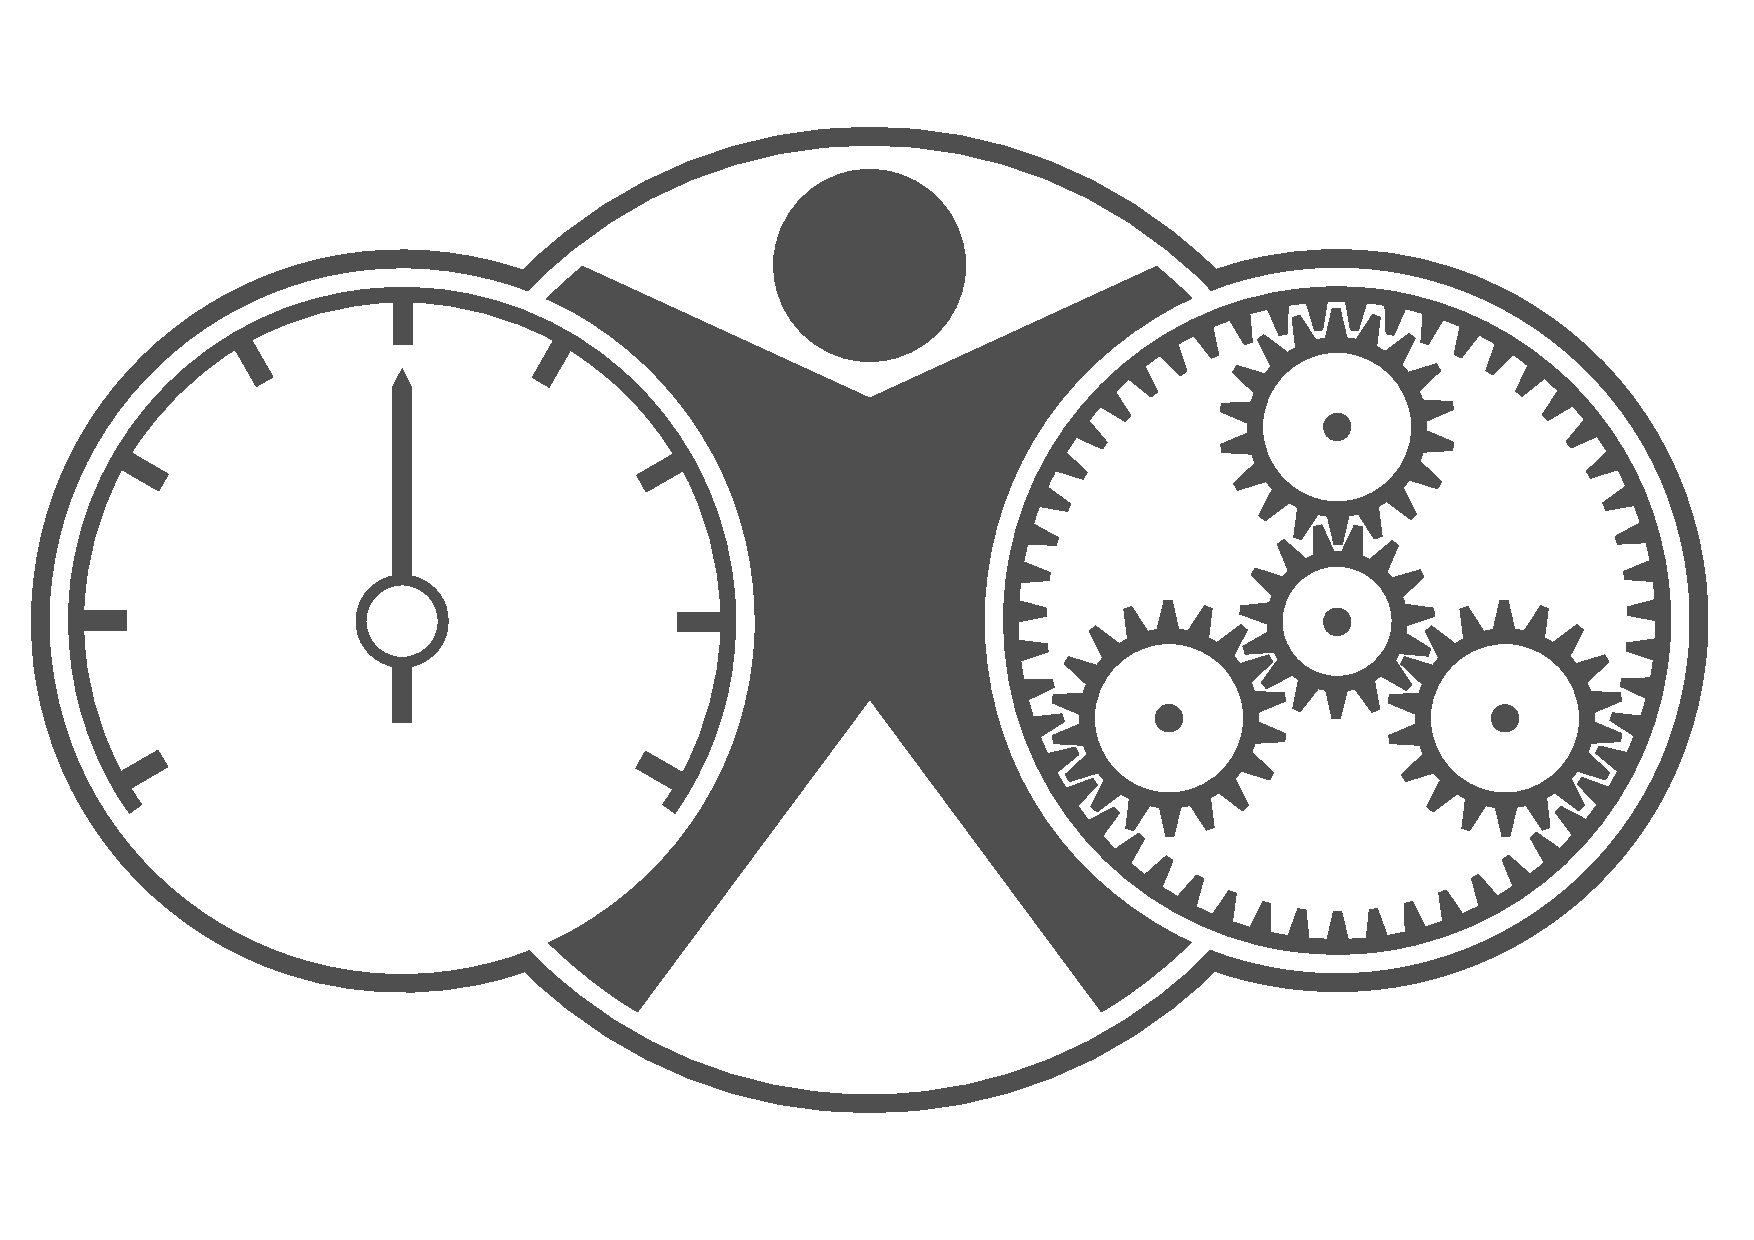
\includegraphics[width=2.5cm]{img/lfe.pdf}
			\end{minipage}
   
%   } 

   \hspace{7cm}
   
   %\put(0,0){
			\begin{minipage}[ht]{0.3\textwidth}
			\centering
			
\includegraphics[width=2.3cm]{img/tum.png}
			\end{minipage}
	}   
\end{picture} \\


\ \\
Technische Universit�t M�nchen\\
Lehrstuhl f�r Ergonomie 

\vspace{3cm}


{\Large\bf \mythema}\\

{\large\bf \mythemaeng}\\

\vspace{1cm}

{\large \myarbeit}\\

\vspace{1cm}


\begin{table}[!hbt]
\large
		\begin{tabular}{ll}
      \vspace{0.5cm}
				Verfasser: & \myname\\
      \vspace{0.5cm}
				Module: & \mymodul\\
      \vspace{0cm}
				Betreuer:	&Univ.-Prof. Dr. phil. Klaus Bengler\\
			\vspace{0cm}
									&Dipl.-Ing. N. N.\\
			\vspace{0.5cm}
									&Dipl.-Inf. N. N.\\						
      \vspace{0.5cm}
				Ausgabe am:&01.01.2012\\
      \vspace{0.5cm}
				Abgabe am:&30.06.2012\\    		
		\end{tabular}
    \vspace{1ex}
\end{table}

 %---------- Bitte anpassen! ----------

\clearpage

\noindent{\Large\bf Eidesstattliche Erkl�rung }\\
\\
Hiermit versichere ich diese Studienarbeit ohne fremde Hilfe selbst�ndig verfasst und nur die angegebenen Quellen und Hilfsmittel verwendet zu haben. W�rtlich oder dem Sinn nach aus anderen Werken entnommene Stellen sind unter Angabe der Quellen kenntlich gemacht.\\
\\
Garching, den\vspace{2.5cm}\\\myname\\

\vspace{3cm}

\noindent{\Large\bf Vereinbarung zum Urheberrecht}\\
\\
Hiermit gestatte ich dem Lehrstuhl f�r Ergonomie diese Studienarbeit bzw. Teile davon nach eigenem Ermessen an Dritte weiterzugeben, zu ver�ffentlichen oder anderweitig zu nutzen. Mein pers�nliches Urheberrecht ist �ber diese Regelung hinaus nicht beeintr�chtigt. 

Eventuelle Geheimhaltungsvereinbarungen �ber den Inhalt der Arbeit zwischen mir bzw. dem Lehrstuhl f�r Ergonomie und Dritten bleiben von dieser Vereinbarung unber�hrt.\\
\\
Garching, den\vspace{2cm}\\\myname
 %Erkl�rungen, wird automatisch erstellt




% --------------------------------------------------
% -------------------- ABSTRACT --------------------
% --------------------------------------------------



\begin{abstract}
\thispagestyle{plain} %F�gt eine Seitenzahl ein
\ofoot[\pagemark]{\pagemark} %F�gt eine Seitenzahl ein

\noindent{\bf Kurzfassung / Abstract}\\


Ein Abstract ist eine pr�gnante Inhaltsangabe, ein Abriss ohne Interpretation und Wertung einer wissenschaftlichen Arbeit. In DIN 1426 wird das (oder auch der) Abstract als Kurzreferat zur Inhaltsangabe beschrieben.

Die Definition des American National Standards Institute (ANSI) lautet: "An abstract is defined as an abbreviated accurate representation of the contents of a document." ("Ein Abstract ist definiert als eine gek�rzte pr�zise Darstellung des Inhalts eines Dokuments.")


\end{abstract}




% --------------------------------------------------
% --------------- INHALTVERZEICHNIS ----------------
% --------------------------------------------------



\tableofcontents %Bindet das Inhaltsverzeichnis ein

\thispagestyle{plain} %F�gt eine Seitenzahl ein
\ofoot[\pagemark]{\pagemark} %F�gt eine Seitenzahl ein

\clearpage

\phantomsection

\clearpage

\setcounter{page}{4} %Seitenz�hler resetten

% --------------------------------------------------
% ------------------- HAUPTTEIL --------------------
% --------------------------------------------------



\newpage{\pagestyle{plain}
\cleardoublepage}
\renewcommand{\thepage}{\arabic{page}}
\setcounter{page}{1}
\pagestyle{scrheadings}
\renewcommand*{\chapterpagestyle}{scrheadings}

%Es bietet sich an, die einzelnen Kapitel in eigene *.tex Dateien auszulagern, um die �bersichtlichkeit zu verbessern. Sollte das nicht gew�nscht sein, k�nnen die Inhalte dieser *.tex Dateien hier eingef�gt und die "\input xxx.tex"' zeilen entfernt werden.
%Die Gliederung/Kapitel ist/sind nat�rlich der Arbeit entsprechend anzupassen

\chapter{Introduction} \label{cha:introduction}

In the development of new interfaces for the vehicles, or simply in the study of 
the influence in driving performance of some factor of interest, an evaluation
has to be performed. There are different ways to measure the driving quality of
a person under the interest conditions. In particular, there are two important
measurements for this task, the Time to Headway (THW) and the standard deviation
of lateral position (SDLP).

To calculate these measurements is necessary to use points of reference. In the
case of the Time to Headway the point of reference are the vehicles driving in
front of the testing car. In the case of the SDLP measurement, the lanes on the
road are used as the reference point to obtain the lateral position.

In a virtual environment is easy to obtain the exact position of the vehicles
and the lanes on the road, but in the real world is not an easy task. In real
world applications, sensors are used to estimate the position of these reference
points. Unfortunately, sensor measurements generally have some error associated
which is directly associated to the price of the sensor. Expensive sensors like
for example laser scanners are very accurate for distance calculation but at the
same time their price is very high. On the other hand, normal color cameras are
getting more popular to be used as sensors in real world reconstruction due to
its low cost and the recent advances in Computer Vision and Image Processing.

In particular, in the recent years a great number of applications using the
Smartphones cameras have been created. For example, augmented reality
applications that superpose a virtual environment by building references with
the real world through the camera.

Here is where the idea of using a similar application for the problem of
evaluating the driving quality shows up. In particular, to create an application
that uses the camera together with Computer Vision technique to calculate the
THW and SDLP measurements in real-time.

This project is precisely this idea taken to practice. The goal of the current
work is to develop an application
for the Android operative system used by Smartphones and mobile devices for
calculating these two measurements. The project was divided in two modules, one
for each measurement. The first one is the Vehicle Detection Module and is the
one responsible for calculate the THW. The second one is called Lane Detection
Module and is the responsible for the detection of the road lanes and the SDLP
calculation.



\chapter{Anmerkungen zum Format} \label{kap:anmerkungen}


Tabelle \ref{tbl:tab1} zeigt, dass Tabellen eine kursive �berschrift tagen.


\begin{table}[h]
	\centering
	\caption{\textit{So sieht eine Tabelle aus (Bild)}}
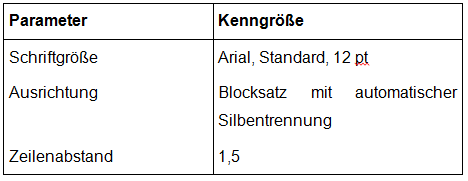
\includegraphics[width=11cm]{img/tabelle.png}
\label{tbl:tab1}
\end{table} 

Tabellen k�nnen entweder als Bild (z.b. aus Excel) eingef�gt werden oder manuell mit LaTeX erstellt werden (siehe \ref{tbl:tab2}):


\begin{table}[h]
	\centering
	\caption{\textit{So sieht eine Tabelle aus (LaTeX)}}	
	\begin{tabular}{|p{3cm}|p{5cm}|}
 			\hline
			\textbf{Parameter} & \textbf{Kenngr��e}\\
			\hline	
				Schriftgr��e & Arial, Standard, 12 pt\\
				Ausrichtung & Blocksatz mit automatischer Silbentrennung\\
				Zeilenabstand & 1,5\\
			\hline
			\end{tabular}
	\label{tbl:tab2}
\end{table} 


Abbildungen tragen eine kursive Bildunterschrift, wie in Abb. \ref{fig:bild1} zu erkennen.

\begin{figure}[ht]
	\centering

\includegraphics[width=8cm]{img/abbildung.png}
\caption{\textit{So sieht eine Abbildung aus}}
\label{fig:bild1}
\end{figure} 

Verweise auf Kapitel, Tabellen oder Abbildungen mit $\backslash ref\{label\}$.



\chapter{Sumatra PDF Viewer}  \label{kap:sumatra}

Statt den Adobe Reader zu verwenden, bietet sich f�r die Arbeit mit TeXnicCenter der Sumatra PDF-Viewer an. Dieser erm�glicht es, das PDF-Dokument w�hrend der Bearbeitung mit TeXnicCenter ge�ffnet zu lassen. Das PDF-Dokument aktuallisiert sich au�erdem nach der Ausgabe automatisch und die Ansicht bleibt an der entsprechenden Stelle im Dokument.\\

Der Sumatra PDF Viewer ist Freeware und sehr schlank.
Er liegt dieser Vorlage als "SumatraPDF-2.1.1-install.exe" bei, oder steht
auf der Seite des Herstellers zum Download bereit:\\

http://blog.kowalczyk.info/software/sumatrapdf/download-free-pdf-viewer-de.html \\

Nach der Installation muss noch die Einstellung des TeXnixCenter f�r die Verwendung von Sumatra angepasst werden.

Eine Anleitung findet sich in "Sumatra Einrichtung.pdf" oder hier:\\

http://www.texniccenter.org/resources/tutorials


%ERGEBNISSE

\chapter{Bibtex, Citavi und Zitieren} \label{kap:bibtex}
Diese LaTeX-Vorlage verwendet Bibtex zur einfachen Darstellung eines Literaturverzeichnisses.

Es gibt verschiedene Editoren f�r Bibtex Dateien, z.B. JabRef.

Wird mit Citavi gearbeitet, so kann die Literatur automatisch in eine Bibtex-Datei geschrieben werden. \\

Daf�r auf Datei -> Exportieren

\begin{figure}[h]
	\centering
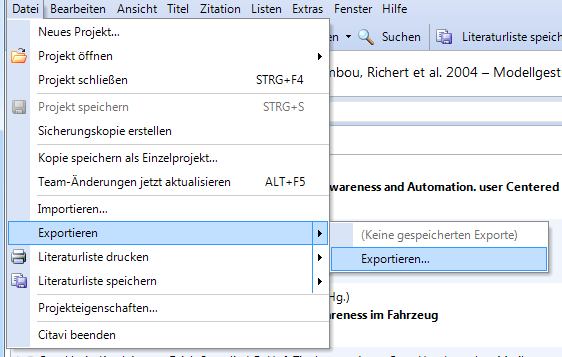
\includegraphics[width=12cm]{img/bib1.png}
\caption{\textit{Exportieren}}
\label{fig:bib1}
\end{figure} 

Im n�chsten Fenster auf "Alle XX Titel in diesem Projekt" und "Weiter".\\

Anschlie�end "BibTeX" anw�hlen und "Weiter".

\begin{figure}[!ht]
	\centering
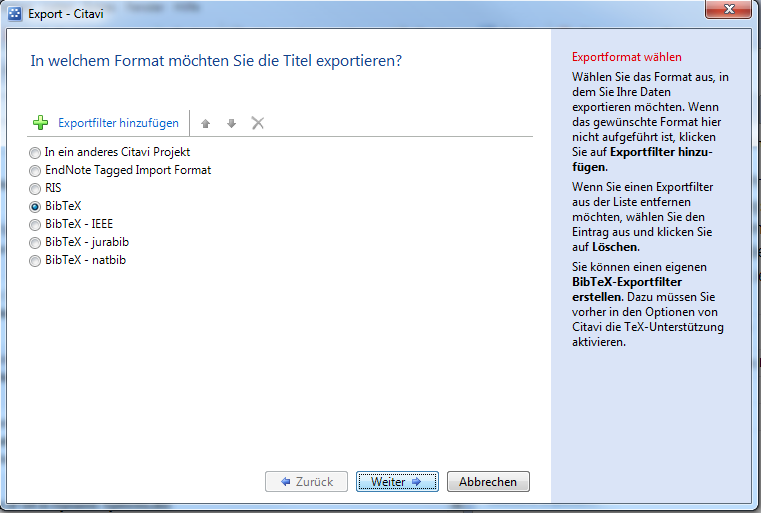
\includegraphics[width=13cm]{img/bib2.png}
\caption{\textit{Fomart zum Exportieren}}
\label{fig:bib2}
\end{figure} 

Jetzt die entsprechende *.bib Datei ausw�hlen. Diese sollte in dem Projektordner liegen und Bibtex.bib hei�en. F�r einen anderen Ort oder Dateinamen muss "$\backslash$bibliography\{Bibtex\}" im "Studienarbeit.tex" entsprechend angepasst werden.
Au�erdem einen Haken bei "Bibtex-Datei aktualisieren".

\begin{figure}[!ht]
	\centering
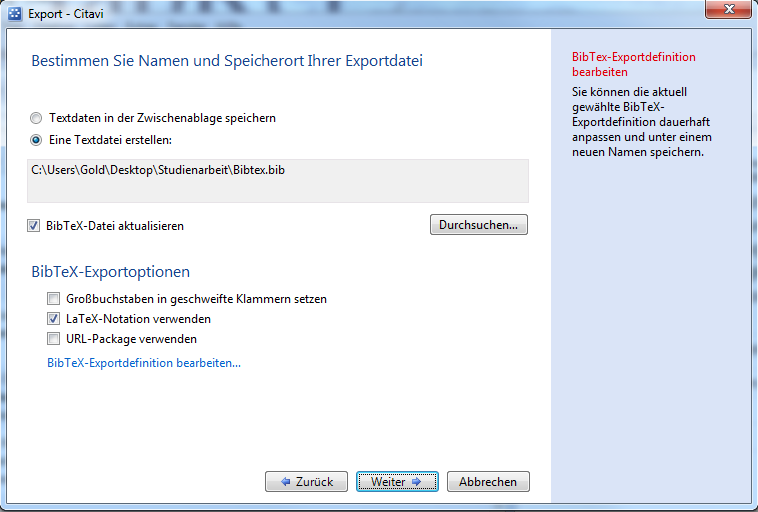
\includegraphics[width=13cm]{img/bib3.png}
\caption{\textit{Datei ausw�hlen}}
\label{fig:bib3}
\end{figure} 

Im n�chsten Fenster der Exportvorlage einen Namen geben und einen Haken bei "Automatisch exportieren beim Speichern" setzen. 

\begin{figure}[ht]
	\centering
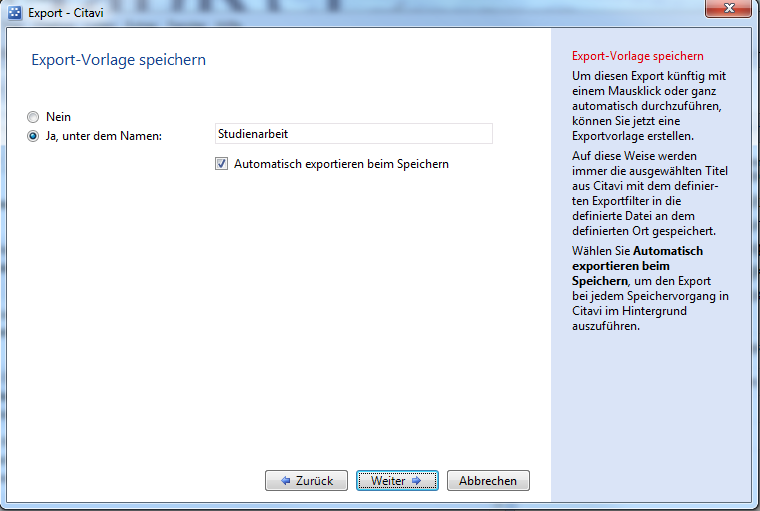
\includegraphics[width=13cm]{img/bib4.png}
\caption{\textit{Automatisch aktualisieren}}
\label{fig:bib4}
\end{figure} 

Bei jeder �nderung in Citavi aktualisiert sich die Bibtex-Datei automatisch mit und ist somit immer auf dem aktuellstem Stand. 

Die gesamte in Citavi gespeicherte Literatur steht nun zum zitieren bereit und es kann mit "$\backslash$cite\{Name.Jahr\}" eine Literaturangabe gesetzt werden. Damit alle Zitate und Seitenzahlen stimmen, muss das Projekt am Ende mehrfach kompiliert werden.\\

Beispiel:

So sagte \cite{Mustermann.2012}, dass... bzw. "Ich bin klug" \citep{Mustermann.2012}.





% --------------------------------------------------
% -------------- LITERATURVERZEICHNIS --------------
% --------------------------------------------------
	
	
\bibliographystyle{apalike} %Zitierstil wie APA6
\bibliography{Bibtex} %Bibliotheksdatei, hier Bibtex.bib



% --------------------------------------------------
% ------------------ VERZEICHNISSE -----------------
% --------------------------------------------------


\listoffigures %Abbildungsverteichnis
\listoftables %Tabellenverzeichnis



% --------------------------------------------------
% --------------------- GOSSAR ---------------------
% --------------------------------------------------


%Sollte ein Glossar erw�nscht sein:
\addcontentsline{toc}{chapter}{Glossar}
\chapter*{Glossar}
\begin{tabbing}
\hspace{3cm} \= \hspace{10cm} \kill \\
MfG \> Mit freundlichen Gr��en\\
\end{tabbing}
 %Bitte bearbeiten




% --------------------------------------------------
% -------------------- ANHANG ----------------------
% --------------------------------------------------


\begin{appendix} %Anhang
\refstepcounter{chapter}
\addchap{Anhang}
Anhang A 

\end{appendix}

\end{document}

% --------------------------------------------------
% --------------------------------------------------
% --------------------------------------------------